\subsubsection{Aut\'omatas celulares de una dimensi\'on}
\label{sec:AutomatasCel1D}
%Parrafo 1
    Los aut\'omatas celulares de una dimensi\'on consisten de una linea de celdas o estados, cada una con 2 estados posibles, 
        0 o 1, vivo o muerto, etc. Estas celdas se actualizan en cada generaci\'on, de acuerdo a una regla de evoluci\'on, 
        la cual determina el estado de una celda en la siguiente generaci\'on, bas\'andose en el estado de la celda y sus 
        vecinos en la generaci\'on actual. La regla de evoluci\'on se aplica a todas las celdas de la misma manera, y en 
        paralelo, es decir, todas las celdas se actualizan al mismo tiempo. Para ejemplificar esto, se puede ver la Figura
        \ref{fig:automataCelular1D}. En donde tenemos la regla de evoluci\'on 30, de las \textit{Reglas de Wolfram}\cite{Wolfram1959}, o
        \textit{Elementary Cellular Automata} (ECA), en la cual se puede ver que la celda de la generaci\'on $t+1$ depende
        de la celda de la generaci\'on $t$ y sus vecinos.
        \begin{figure}[h!]
            \centering
            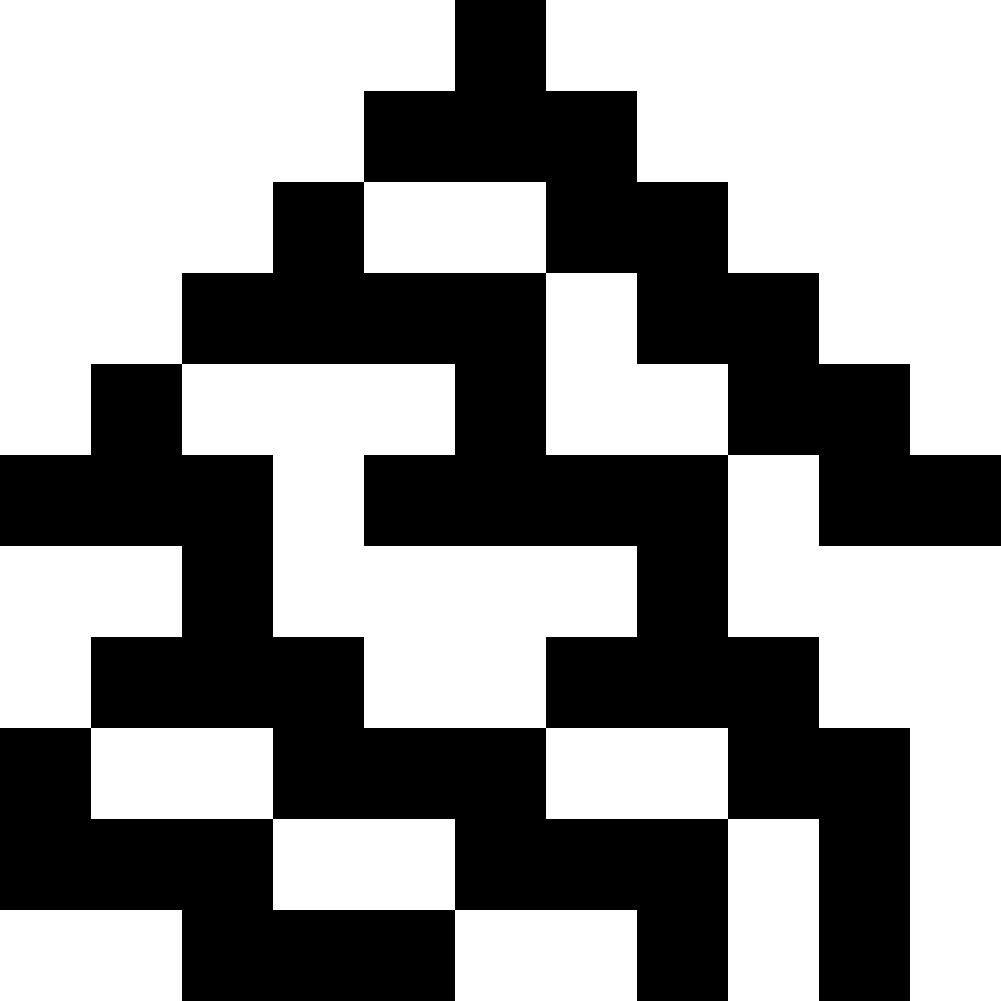
\includegraphics[width=0.5\textwidth]{./images/marco_teorico/automatas_celulares/Regla30.png}
            \caption{Regla de evoluci\'on 30 de las \textit{Reglas de Wolfram} 10 generaciones o (t)}
            \label{fig:automataCelular1D}
        \end{figure}
%Parrafo 2
    \vskip 0.5cm
    Como podemos ver en estos aut\'omatas celulares de una dimensi\'on los que podemos considerar los elementos m\'as importantes son:
        \begin{itemize}
            \item \textbf{Vecindad:} Es el conjunto de celdas que se toman en cuenta para la actualizaci\'on de una celda.
            \item \textbf{Estado:} Es el valor que puede tomar una celda, en este caso solo puede ser 0 o 1.
            \item \textbf{Regla de evoluci\'on:} Es la regla que determina el estado de una celda en la siguiente generaci\'on.
        \end{itemize}
    \vskip 0.5cm
    En este caso la vecindad la forman la celda y sus dos vecinos, pero puede ser de cualquier tama\~no, siempre y cuando
        sea sim\'etrica, es decir, que la celda se encuentre en el centro de la vecindad. El estado de la celda puede ser
        cualquier valor, pero en este caso solo puede ser 0 o 1. La regla de evoluci\'on es la que determina el estado de
        la celda en la siguiente generaci\'on, en este caso la regla de evoluci\'on 30, que se puede ver en la Figura
        \ref{fig:automataCelular1D}, es la siguiente:
        \begin{table}[h!]
            \centering
            \begin{tabular}{|c|c|c|c|c|c|c|c|}
                \hline
                \textbf{111} & \textbf{110} & \textbf{101} & \textbf{100} & \textbf{011} & \textbf{010} & \textbf{001} & \textbf{000} \\
                \hline
                0 & 0 & 0 & 1 & 1 & 1 & 1 & 0 \\
                \hline
            \end{tabular}
            \caption{Regla de evoluci\'on 30}
            \label{tab:reglaEvolucion30}
        \end{table}
    \vskip 0.5cm
    Como podemos ver en el Cuadro \ref{tab:reglaEvolucion30} la regla de evoluci\'on 30 es una regla de evoluci\'on local, 
        es decir, que solo depende de la celda y sus vecinos, y no de toda la l\'inea de celdas. En este caso la regla de evoluci\'on
        30 es una regla de evoluci\'on determinista, es decir, que para una celda y sus vecinos siempre se obtiene el mismo resultado.
        Pero tambi\'en existen las reglas de evoluci\'on no deterministas, en las cuales para una celda y sus vecinos se puede obtener
        m\'as de un resultado. En este caso la regla de evoluci\'on 30 es una regla de evoluci\'on unidimensional, es decir, que la
        celda solo depende de sus vecinos de la izquierda y de la derecha, pero tambi\'en existen las reglas de evoluci\'on
        bidimensionales, n-dimensionales, etc.
    \vskip 0.5cm
    \subsubsection{Condiciones frontera}
        Por definici\'on los aut\'omatas celulares son infinitos, pero en la pr\'actica no se pueden tener aut\'omatas celulares
            infinitos, por lo que se tienen que definir condiciones frontera, las cuales son las condiciones que se tienen en los
            extremos del aut\'omata celular. Existen diferentes tipos de condiciones frontera, las cuales son:
            \vskip 0.5cm
        \begin{wrapfigure}{r}{0.25\textwidth}
            \centering
            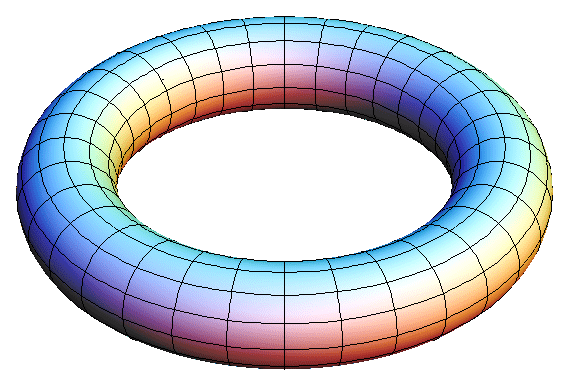
\includegraphics[width=0.25\textwidth]{./images/marco_teorico/automatas_celulares/torus.png}
            \caption{Representaci\'on de un toroide \cite{Sharma2022}}
            \label{fig:toroide}
        \end{wrapfigure}
        \begin{itemize}
            \item \textbf{Abierta} En este caso las celdas de los extremos no tienen vecinos, por lo que no se pueden actualizar.
            \item \textbf{Peri\'odica} En este caso las celdas de los extremos tienen como vecinos a las celdas del otro extremo.
            \item \textbf{Reflejante} En este caso las celdas de los extremos tienen como vecinos a las celdas del otro extremo, pero
                invertidas.
            \item \textbf{Frontera} En este caso las celdas de los extremos tienen como vecinos a celdas con un valor fijo.
        \end{itemize}
    \vskip 0.5cm
    En nuestro caso, utilizaremos la condici\'on frontera peri\'odica; esta tiene forma de un toroide, como se puede ver en la Figura
        \ref{fig:toroide}.
        \vskip 0.5cm
        
        Tambi\'en podemos observar que en la Figura \ref{fig:toroide} se puede ver que las celdas de los extremos tienen como
            vecinos a las celdas del otro extremo, por lo que se puede decir que es una condici\'on frontera peri\'odica.
        \vskip 0.5cm